\chapter{Les triangles dont les aires et les périmètres sont égaux sont-ils isométriques ?}\label{c.congruent}

%%%%%%%%%%%%%%%%%%%%%%%%%%%%%%%%%%%%%%%%%%%%%%%%%%%%%%%%%%%%%%%


Deux triangles ayant la même aire et le même périmètre sont-ils isométriques ? Pas nécessairement : les triangles de côtés $(17,25,28)$ et $(20,21,29)$ ont tous deux un périmètre de $70$ et une aire de $210$ mais ils ne sont pas isométriques (fig.~\ref{f.congruent-first-example}).\footnote{Les aires ont été calculées à l'aide de la formule de Héron (théorème~\ref{thm.heron}) et les angles à l'aide de la loi des cosinus (théorème~\ref{thm.law-of-cosines}).} Ce chapitre montre qu'à partir d'un triangle à côtés rationnels, il est possible de construire un triangle non isométrique, également à côtés rationnels, qui a la même aire et le même périmètre.
Nous menons la déduction à l'aide d'un exemple, en montrant que le triangle de côtés $(3,4,5)$ et le triangle de côtés 
$\left(\frac{156}{35}, \frac{101}{21}, \frac{41}{15}\right)$  ont tous deux un périmètre de $12$ et une aire de $6$.

\begin{figure}[htbp]
\centering
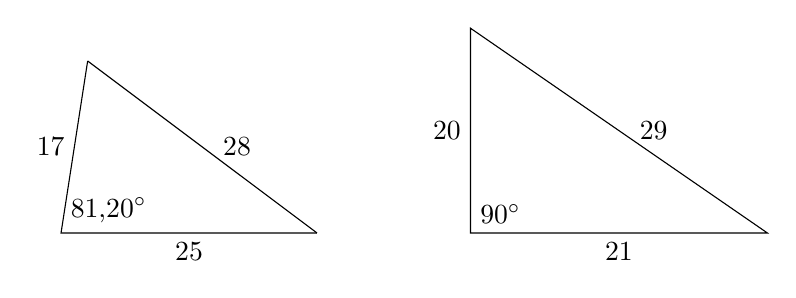
\begin{tikzpicture}[scale=1.3]
\coordinate (A1) at (0,0);
\node[above right] at (A1) {$\mbox{81,20}^\circ$};
\coordinate (B1) at (2.5cm,0);
\coordinate (C1) at (81.20:1.7cm);
\draw (B1) -- node[below] {$25$} (A1) -- node[left] {$17$} (C1);
\draw (B1) -- node[right,xshift=4pt] {$28$} +(143.13:2.8cm);
\begin{scope}[xshift=4cm]
\coordinate (A2) at (0,0);
\node[above right] at (A2) {$90^\circ$};
\coordinate (B2) at (2.9cm,0);
\coordinate (C2) at (0,2cm);
\draw (B2) -- node[below] {$21$} (A2) -- node[left] {$20$} (C2) -- node[right,xshift=4pt] {$29$} cycle;
\end{scope}
\end{tikzpicture}
%\includegraphics[width=\textwidth]{Fig15_1}

\caption{Triangles non isométriques ayant la même aire et le même périmètre.}\label{f.congruent-first-example}
\end{figure}


\section{D'un triangle à une courbe elliptique}\label{s.elliptic}

Les trois bissectrices des angles d'un triangle se coupent en un point $O$ qui est le centre du cercle inscrit dans le triangle (fig.~\ref{f.congruent1}). 

Traçons les hauteurs du centre $O$ vers les côtés. Les hauteurs ont une longueur $r$, le rayon du cercle inscrit. Les hauteurs et les bissectrices des angles créent trois paires de triangles rectangles isométriques :
\[
\triangle AOB'\cong \triangle AOC',\quad \triangle BOA'\cong \triangle BOC',\quad \triangle COA'\cong \triangle COB'\,.
\]

\begin{figure}[htbp]
\centering
\begin{tikzpicture}[scale=1.75]
% Draw base and path two lines at known angles
\draw (0,0) coordinate (a) node[below] {$A$} --
  (0:6) coordinate (b) node[below] {$B$};
\path[name path=ac] (a) -- +(50:4);
\path[name path=bc] (b) -- +(150:5);
% Get their intersection and draw lines between vertices
\path[name intersections={of=ac and bc,by=c}];
\node[above] at (c) {$C$};
\draw (a) -- (c) -- (b) -- (a);
% Label angles with tick marks
\draw (a) ++(0:4mm) arc (0:50:4mm);
\draw (a) ++(10:3.5mm) -- +(10:1mm);
\draw (a) ++(15:3.5mm) -- +(15:1mm);
\draw (a) ++(35:3.5mm) -- +(35:1mm);
\draw (a) ++(40:3.5mm) -- +(45:1mm);
\draw (b) ++(150:5mm) arc (150:180:5mm);
\draw (b) ++(157.5:4.5mm) -- +(157.5:1mm);
\draw (b) ++(172.5:4.5mm) -- +(172.5:1mm);
\draw (c) ++(230:3mm) arc (230:330:3mm);
\draw (c) ++(250:2.5mm) -- +(250:1mm);
\draw (c) ++(255:2.5mm) -- +(255:1mm);
\draw (c) ++(260:2.5mm) -- +(260:1mm);
\draw (c) ++(300:2.5mm) -- +(300:1mm);
\draw (c) ++(305:2.5mm) -- +(305:1mm);
\draw (c) ++(310:2.5mm) -- +(310:1mm);
% Path bisectors of two lines
\path[name path=bia] (a) -- +(25:3.5);
\path[name path=bib] (b) -- +(165:5);
% Intersection of angle bisectors
\path [name intersections={of=bia and bib,by=center}];
% Draw angle bisectors to center
\draw (a) -- (center);
\draw (c) -- (center);
\draw (b) -- (center);
% Draw radii
\draw (center) -- node[left] {$r$}
  ($(a)!(center)!(b)$) node[below,yshift=-2pt] {$C'$}
  coordinate (ap);
\draw (center) -- node[left,yshift=-4pt] {$r$}
  ($(a)!(center)!(c)$) node[above left,xshift=4pt] {$B'$}
  coordinate (bp);
\draw (center) -- node[right] {$r$}
  ($(b)!(center)!(c)$) node[above right] {$A'$}
  coordinate (cp);
\vertex{center};
\node[above,xshift=3pt,yshift=6pt] at (center) {$O$};
% Draw right angle squares
\draw (ap) rectangle +(3pt,3pt);
\draw[rotate=-40] (bp) rectangle +(3pt,3pt);
\draw[rotate=-120] (cp) rectangle +(3pt,3pt);
% Labels of angles
\node[above,xshift=5pt,yshift=21pt]
  at (center) {$\gamma/2$};
\node[above left,xshift=-4pt,yshift=21pt]
  at (center) {$\gamma/2$};
\node[above right,xshift=4pt,yshift=-5pt]
  at (center) {$\beta/2$};
\node[below right,yshift=-6pt]
  at (center) {$\beta/2$};
\node[left,xshift=-8pt,yshift=3pt]
  at (center) {$\alpha/2$};
\node[below left,xshift=2pt,yshift=-6pt]
  at (center) {$\alpha/2$};
% Labels of line segments (names of points are weird...)
\path (a) -- node[below,yshift=-2pt] {$u$} (ap);
\path (a) -- node[left, xshift=-2pt] {$u$} (bp);
\path (b) -- node[above,yshift=2pt]  {$v$} (cp);
\path (b) -- node[below,xshift=-2pt] {$v$} (ap);
\path (c) -- node[above,xshift=-2pt] {$w$} (bp);
\path (c) -- node[above,xshift=2pt]  {$w$} (cp);
% Labels of sides
\draw[<->] ($(a)+(0,-10pt)$) -- node[fill=white] {$c$} 
           ($(b)+(0,-10pt)$);
\draw[<->] ($(a)+(-4pt,7pt)$) -- node[fill=white] {$b$}
           ($(c)+(-4pt,7pt)$);
\draw[<->] ($(b)+(2pt,9pt)$) -- node[fill=white] {$a$}
           ($(c)+(2pt,9pt)$);
% Inscribed circle
\node[draw,circle through=(ap)] at (center) {};
\end{tikzpicture}
%\includegraphics[width=\textwidth]{Fig15_2}
\caption{Le cercle inscrit dans un triangle.}\label{f.congruent1}
\end{figure}

Les hauteurs divisent les côtés $a$, $b$ et $c$ en segments $u$, $v$ et $w$. L'aire du triangle ABC est la somme des aires de $\triangle BOC$, $\triangle AOB$ et $\triangle AOC$ :
%
\begin{subequations}
\begin{align}
A &= \frac{1}{2}(w+v)r + \frac{1}{2}(v+u)r + \frac{1}{2}(u+w)r\\
&=\frac{1}{2}\cdot 2(u+v+w)r\\
&=\frac{1}{2}(a+b+c)r\\
&=sr\,, \slabel{eq.area1}
\end{align}
\end{subequations}
où $s$ est le demi-périmètre, la moitié du périmètre du triangle $\triangle ABC$. Les longueurs  $u$, $v$ et $w$ s'expriment à l'aide du rayon du cercle et des angles centraux 
 $\alpha/2$, $\beta/2$ et $\gamma/2$:
\begin{align}
\tan \frac{\alpha}{2}= \frac{u}{r},\quad
\tan \frac{\beta}{2} = \frac{v}{r},\quad
\tan \frac{\gamma}{2} =\frac{w}{r}\,.\label{eq.uvw}
\end{align}
Le demi-périmètre peut maintenant être exprimé en fonction des tangentes :
\[
s = u+v+w = r\tan \frac{\alpha}{2}+r\tan \frac{\beta}{2}+r\tan \frac{\gamma}{2} = r\left(\tan \frac{\alpha}{2}+\tan \frac{\beta}{2}+\tan \frac{\gamma}{2}\right).
\]
D'après l'équation~\ref{eq.area1},  l'aire est 
\begin{align}
A = sr = r^2\left(\tan \frac{\alpha}{2}+\tan \frac{\beta}{2}+\tan \frac{\gamma}{2}\right)\,.\label{eq.area2}
\end{align}
\`A partir de $r=A/s$, l'équation~\ref{eq.area2} peut s'écrire
\begin{align}
\tan \frac{\alpha}{2}+\tan \frac{\beta}{2}+\tan \frac{\gamma}{2} = \frac{A}{r^2} = \frac{A}{(A/s)^2} = \frac{s^2}{A}\,.\label{eq.area3}
\end{align}
Puisque la somme des angles $\alpha$, $\beta$ et $\gamma$ est $360^\circ$,
%
\begin{subequations}
\begin{align}
\gamma/2 &= 360^\circ/2 - (\alpha/2 + \beta/2)\\
\tan\gamma/2 &= \tan(180^\circ - (\alpha/2 + \beta/2))\\
 &= -\tan (\alpha/2 + \beta/2)\\
&= \frac{\tan\alpha/2 + \tan\beta/2}{\tan\alpha/2 \, \tan\beta/2-1}\,,\slabel{eq.tangent1}
\end{align}
\end{subequations}
en utilisant la formule de la tangente de la somme de deux angles (théorème~\ref{thm.tangent-sum}).

Simplifions les notations en posant 
\begin{align}
x=\tan \frac{\alpha}{2},\quad
y=\tan \frac{\beta}{2},\quad
z=\tan \frac{\gamma}{2}\,.\label{eq.variables-for-tangents}
\end{align}
D'après l'équation~\ref{eq.tangent1},  nous pouvons exprimer $z=\tan\gamma/2$ en fonction de $x$ et $y$ :
\begin{align}
z = \frac{x+y}{xy-1}\,.\label{eq.xy1}
\end{align}
Avec cette notation, l'équation~\ref{eq.area3} devient 
\begin{align}
x+y+\frac{x+y}{xy-1}=\frac{s^2}{A}\,.\label{eq.xy2}
\end{align}
Pour des valeurs fixes de $A$ et $s$, existe-t-il des solutions multiples de l'équation~\ref{eq.xy2} ?

Pour le triangle rectangle $(3,4,5)$,
\begin{align}
\frac{s^2}{A} = \frac{\left(\frac{1}{2}(3+4+5)\right)^2}{\frac{1}{2}\cdot 3\cdot 4} = \frac{6^2}{6}=6\,.
\end{align}
S'il existe une autre solution de l'équation~\ref{eq.xy2} avec $s^2/A=6$, elle peut s'écrire 
\begin{subequations}
\begin{align}
x+y+\frac{x+y}{xy-1}&=6\\
x^2y + xy^2 -6xy + 6 &= 0\,.\slabel{eq.elliptic}
\end{align}
\end{subequations}
C'est l'équation d'une courbe elliptique.

\section{Résolution de l'équation pour la courbe elliptique}

Une partie du graphe de l'équation~\ref{eq.elliptic} est représentée dans la figure~\ref{f.two-secants}. Tout point de la courbe fermée du premier quadrant est une solution de l'équation car les longueurs des côtés du triangle doivent être positives. $A$, $B$ et $D$ correspondent au triangle $(3,4,5)$ comme indiqué ci-dessous. Pour trouver d'autres solutions rationnelles, on utilise la méthode des deux sécantes.

Construisons une sécante passant par les points $A=(2,3)$ et $B=(1,2)$. Elle coupe la courbe en $C=(-\mbox{1,5}\,;\,-\mbox{0,5})$, mais cela ne donne pas de solution car les valeurs sont négatives. Construisons une deuxième sécante de $C$ à $D=(3,2)$. L'intersection avec la courbe en $E\approx (\mbox{1,5}\,;\,\mbox{1,2})$ donne une nouvelle solution dont les coordonnées seront calculées ci-dessous.

\begin{figure}[thbp]
\centering
\begin{tikzpicture}[scale=0.9]
\draw[very thin,step=10mm] (-4,-4) grid (4,4);
\draw[thick] (-4,0) -- (4,0);
\draw[thick] (0,-4) -- (0,4);
\foreach \x in {-3,...,4}
  \node at (\x-.2,-.2) {\sm{\x}};
\foreach \y in {-3,...,-1}
  \node at (+.2,\y-.3) {\sm{\y}};
\foreach \y in {1,...,4}
  \node at (+.2,\y-.3) {\sm{\y}};

\draw[very thick,domain=.936:3.306,samples=200] plot (\x,{
(
  (6*\x-\x*\x)+
  sqrt(
   (\x*\x-6*\x)^2 -
   4*\x*6
  )
)/
(2*\x)
});

\draw[very thick,domain=.936:3.306,samples=100] plot (\x,{
(
  (6*\x-\x*\x)-
  sqrt(
   (\x*\x-6*\x)^2 -
   4*\x*6
  )
)/
(2*\x)
});

\draw[very thick,domain=-2.5:-.25,samples=100] plot (\x,{
(
  (6*\x-\x*\x)+
  sqrt(
   (\x*\x-6*\x)^2 -
   4*\x*6
  )
)/
(2*\x)
});

\coordinate (A) at (2,3);
\coordinate (B) at (1,2);
\coordinate (C) at (-1.5,-0.5);
\coordinate (D) at (3,2);
\coordinate (E) at (1.5,1.2);

\draw[very thick,dashed,red]  ($(C)!-.4!(A)$) -- ($(C)!1.2!(A)$);
\draw[very thick,dashed,blue] ($(C)!-.4!(D)$) -- ($(C)!1.2!(D)$);

\node[right,xshift=9pt,yshift=-5pt]  at (A)  {$A=(2,3)$};
\node[above left,xshift=-4pt]        at (B)  {$B=(1,2)$};
\node[right,xshift=23pt,yshift=-4]   at (C)  {$C=(-\mbox{1,5};-\mbox{0,5})$};
\node[right,xshift=8pt,yshift=-6pt]  at (D)  {$D=(3,2)$};
\node[below,xshift=15pt,yshift=-12pt] at (E) {$E=(\mbox{1,5};\mbox{1,2})$};
\vertexcolor{A}{red};
\vertexcolor{B}{red};
\vertexcolor{C}{purple};
\vertexcolor{D}{blue};
\vertexcolor{E}{blue!50!red};
\end{tikzpicture}
%\includegraphics[width=\textwidth]{Fig15_3}

\caption{La méthode des deux sécantes.}\label{f.two-secants}
\end{figure}


L'équation de la droite (rouge) qui passe par $A$ et $B$ est $y=x+1$. D'après l'équation~\ref{eq.elliptic},
\begin{align*}
x^2(x+1) + x(x+1)^2 -6x(x+1) +6 &=0\\
2x^3 -3x^2 -5x +6 &=0\,.
\end{align*}
Avec $A$ et $B$, on connaît deux racines $x=2$ et $x=1$,  donc on peut factoriser le polynôme de degré trois :
\[
(x-2)(x-1)(ax+b)=0\,,
\]
où la troisième racine est inconnue. Multiplions les facteurs et concluons que $a=2$ et $b=3$ puisque $2x^3 -3x^2 -5x +6 = ax^3+\cdots+2b$. Le troisième facteur est $2x+3$ ce qui donne la troisième racine $x=-\frac{3}{2}$ et $y=x+1=-\frac{1}{2}$. C'est le point $C=(-\frac{3}{2},-\frac{1}{2})$ du graphe.

L'équation de la droite (bleue) qui passe par $C$ et $D$ est 
\begin{align}
y = \frac{5}{9}x + \frac{1}{3}\,.\label{eq.second-secant}
\end{align}
On remplace $y$ dans l'équation~\ref{eq.elliptic}:
\begin{align*}
x^2\left(\frac{5}{9}x + \frac{1}{3}\right) + x\left(\frac{5}{9}x + \frac{1}{3}\right)^2 -6x\left(\frac{5}{9}x + \frac{1}{3}\right) +6 &=0\\
\frac{70}{81}x^3 - \frac{71}{27}x^2 - \frac{17}{9}x +6 &=0\,.
\end{align*}
Avec $C$ et $D$, on connaît deux racines $x=3$ et $x=-\frac{3}{2}$, donc on peut factoriser le polynôme de degré trois :
\[
(x-3)\left(x+\frac{3}{2}\right)(ax+b)=0\,.
\]
En égalant les coefficients du terme de degré trois et du terme constant, on obtient 
\begin{align*}
\frac{70}{81}x - \frac{4}{3}&=0\\
x&= \frac{54}{35}\approx \mbox{1,543}\,,
\end{align*}
et $y$ peut être calculé à partir de l'équation~\ref{eq.second-secant}:
\[
y=\frac{25}{21}\approx \mbox{1,190}\,.
\]
Les coordonnées de $E$ sont 
\[
\left(\frac{54}{35}, \frac{25}{21}\right)=(\mbox{1,543}\,;\,\mbox{1,190})\,,
\]
qui sont proches des approximations $(\mbox{1,5}\,;\,\mbox{1,2})$ obtenues à partir du graphe.

Enfin, calculons $z$ à partir de l'équation~\ref{eq.xy1}:
\[
z=\frac{x+y}{xy-1}=%
\displaystyle\left(\frac{54}{35} + \frac{25}{21}\right)%
 \, \bigg/ \,%
\displaystyle\left(\frac{54}{35}\frac{25}{21}-1\right)=%
\frac{2009}{615} = \frac{49}{15}\,.
\]

\section{Détermination d'un triangle à partir de la courbe elliptique}

\enlargethispage*{\baselineskip}

En utilisant les équations~\ref{eq.uvw} et  \ref{eq.variables-for-tangents},  les côtés $a$, $b$ et $c$ du triangle $\triangle ABC$ peuvent être calculés à partir de $x,y,z$ et $r=A/s=6/6=1$ :
%
\begin{align*}
a&=w+v = r(z+y)=(z+y)\\
b&=u+w= r(x+z)=(x+z)\\
c&=u+v=r(x+y)=(x+y)\,.
\end{align*}
Pour la solution $A$ de la courbe elliptique, les côtés du triangle sont 
\begin{align*}
a &= z+y = 1+3 = 4\\
b &= x+z = 2+1=3\\
c &= x+y = 2+3=5\,.
\end{align*}
Pour la solution $E$ de la courbe elliptique, les côtés du triangle sont 
\begin{align*}
a &= z+y = \frac{49}{15} + \frac{25}{21} = \frac{156}{35}\\
b &= x+z = \frac{54}{35} + \frac{49}{15} = \frac{101}{21}\\
c &= x+y = \frac{54}{35} + \frac{25}{21} =\frac{41}{15}\,.
\end{align*}
Vérifions ce résultat. Le demi-périmètre est 
\[
s=\frac{1}{2}\left(\frac{156}{35} + \frac{101}{21}+\frac{41}{15}\right) = \frac{1}{2}\left(\frac{468+505+287}{105}\right) = \frac{1}{2}\left(\frac{1260}{105}\right)= 6\,,
\]
et l'aire peut être calculée en utilisant la formule de Héron (théorème~\ref{thm.heron}):
\[
A= \sqrt{6 \left(6-\frac{156}{35}\right) \left(6-\frac{101}{21}\right) \left(6-\frac{41}{15}\right)}=\sqrt{36} = 6\,.
\]
Est-ce que $\left(\frac{156}{35}, \frac{101}{21}, \frac{41}{15}\right)\cong(3,4,5)$ ? Pour simplifier le calcul, utilisons les approximations décimales $(\mbox{4,48}\,;\, \mbox{4,81}\,;\, \mbox{2,73})$. Alors 
\[
\sqrt{\mbox{4,48}^2+\mbox{2,73}^2}=\mbox{5,25}\neq \mbox{4,81}\,,
\]
Il ne s'agit donc pas d'un triangle rectangle et il n'est pas isométrique à $(3,4,5)$.

La loi des cosinus peut être utilisée pour calculer les angles du triangle, comme le montre la figure~\ref{f.not-a-right-triangle}.


\begin{figure}[htbp]
\centering

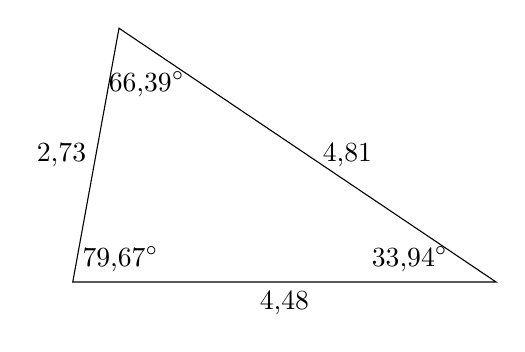
\begin{tikzpicture}[scale=1.2]
\coordinate (A1) at (0,0);
\coordinate (B1) at (4.48cm,0);
\coordinate (C1) at (79.67:2.73cm);
\node[above right] at (A1) {$\mbox{79,67}^\circ$};
\node[above left,xshift=-14pt] at (B1) {$\mbox{33,94}^\circ$};
\node[below,yshift=-12pt,xshift=10pt] at (C1) {$\mbox{66,39}^\circ$};
\draw (B1) -- node[below] {$\mbox{4,48}$} (A1) --
  node[left] {$\mbox{2,73}$} (C1) -- node[right,xshift=2pt] {$\mbox{4,81}$} cycle;
\end{tikzpicture}
%\includegraphics[width=\textwidth]{Fig15_4}
\caption{Le triangle dont le périmètre et l'aire sont identiques à ceux du triangle  $(3,4,5)$.}\label{f.not-a-right-triangle}
\end{figure}



\subsection*{Quelle est la surprise ?}

Les triangles ayant la même aire et le même périmètre sont-ils isométriques ? Ma première impression était de dire \og oui\fg{}, car il n'est pas facile de trouver des contre-exemples. Ce qui est surprenant, c'est qu'étant donné un triangle arbitraire avec des côtés rationnels, il est possible de construire un triangle non congruent avec des côtés rationnels qui a la même aire et le même périmètre, bien que le résultat puisse être étrange comme avec les triangles $(3,4,5)$ et $\left(\frac{156}{35}, \frac{101}{21}, \frac{41}{15}\right)$.



\subsection*{Sources}

Ce chapitre se base sur \cite{mccallum}. Dans \cite{marita}, on montre qu'étant donné un triangle isocèle, il existe des triangles non congruents ayant la même aire et le même périmètre, mais la démonstration ne comporte pas de construction explicite.
